\documentclass{article}
\usepackage{graphicx, xcolor}
\usepackage[a4paper, tmargin=1in, bmargin=1in]{geometry}
\usepackage[utf8]{inputenc}
\usepackage[justification=centering]{caption}

% \usepackage{parskip}
\usepackage{pdflscape}
\usepackage{listings}
\usepackage{hyperref}
\usepackage{caption}
\usepackage{subcaption}
\usepackage{float}

\title{EE739A - Advanced Processor Design\\
  Project I : Superscalar IITB RISC
}
\author{Meet Udeshi - 14D070007\\
  OV Shashank - 14D070021\\
  Arka Sadhu - 140070011\\
}
\date{\today}

\begin{document}
\maketitle

\section{Fetch}
\begin{figure}[H]
	\centering
	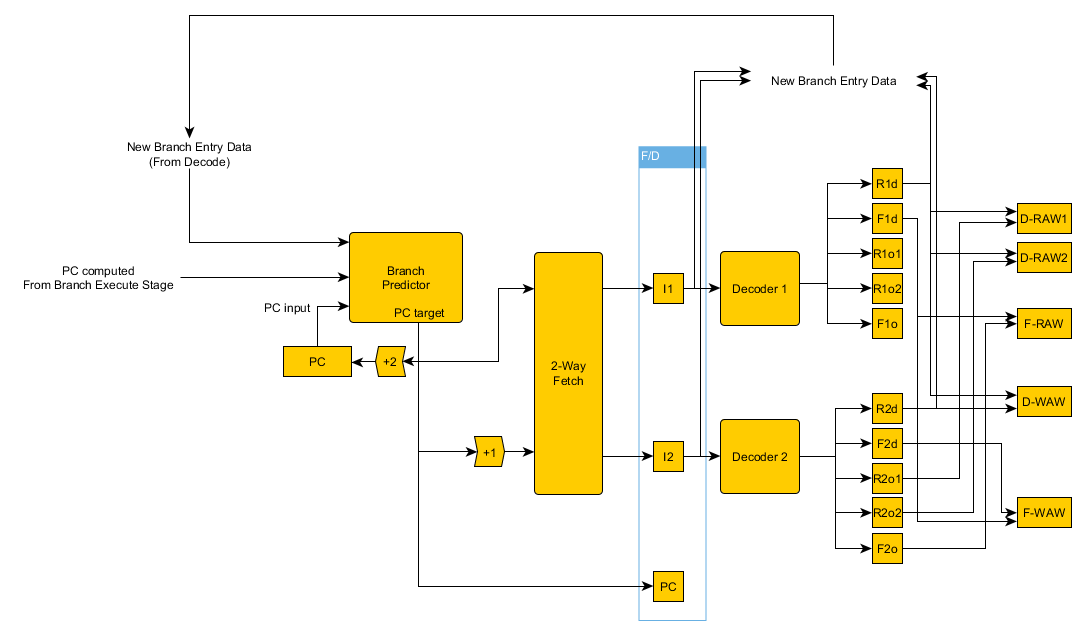
\includegraphics[scale = 0.4]{../GraphImages/fetch_decode.png}
\end{figure}

\subsection{Program Counter}
\begin{itemize}
\item This register is the speculative program counter which is used to fetch from the instruction cache
\item The actual permanent PC is stored in the ARF corresponding to register R7 as R7 == PC in the ISA
\item It is updated by PC+2 every cycle, unless a branch misprediction correction is issued or the fetch stage is stalled
\end{itemize}
\subsection{Branch Predictor (BP)}
\begin{itemize}
\item Stores Target Address and Prediction History corresponding to BEQ, JAL and JLR. Though JLR is a multi-taregted branch, assuming that it would be used much as a multi-target, we predict it using a single BTA. The other R7 write instructions could also be predicted with minimal hardware change, but to prevent BP Pollution we are not including them.
\item JLR is not stores becuase its target address needs to always be computed and can be multitargeted which adds issues in checking whether the branch taken was to the right address or not
\item Branches are by default assumed to be not taken so that PC+2 rule can be continually followed
\item Planned to be implemented as a two bit predictor because the ISA does not allow from good prediction accuracy with small hardware
\end{itemize}

\section{Decode}
\subsection{Decoders}
\begin{itemize}
\item There are two parallel decoders which generate the necessary control signals for the future stages. This also includes the necessary reordering of the operands into source and destination registers
\item They include necessary hardware to detect inter-dependencies between the two instructions fetched
\item They generate inter-dependency bits which are later to be used in the renaming stage by the ARF and RRF to correctly generate and provide the tags
\item The validity of the destination operand for the ARF as well as for the carry and zero flags are produced which is passed on as the invalid tag bits in the execution stage
\end{itemize}
\subsection{LM/SM Handling Block}
\begin{itemize}
\item It is responsible for replacing the decode block in case of arrival of an LM or SM
\item It generates the necessary operands and addresses that are to be written to or read from. This is performed by generating signals similar to the load instruction and simply by incrementing the immediate field
\item To ensure that the value read from Address Source Register does not change an isLM bit is generated which is a signal for harware in the dispatch stange which ensures correct execution of the instruction
\end{itemize}

\section{Dispatch}
\begin{figure}[H]
	\centering
	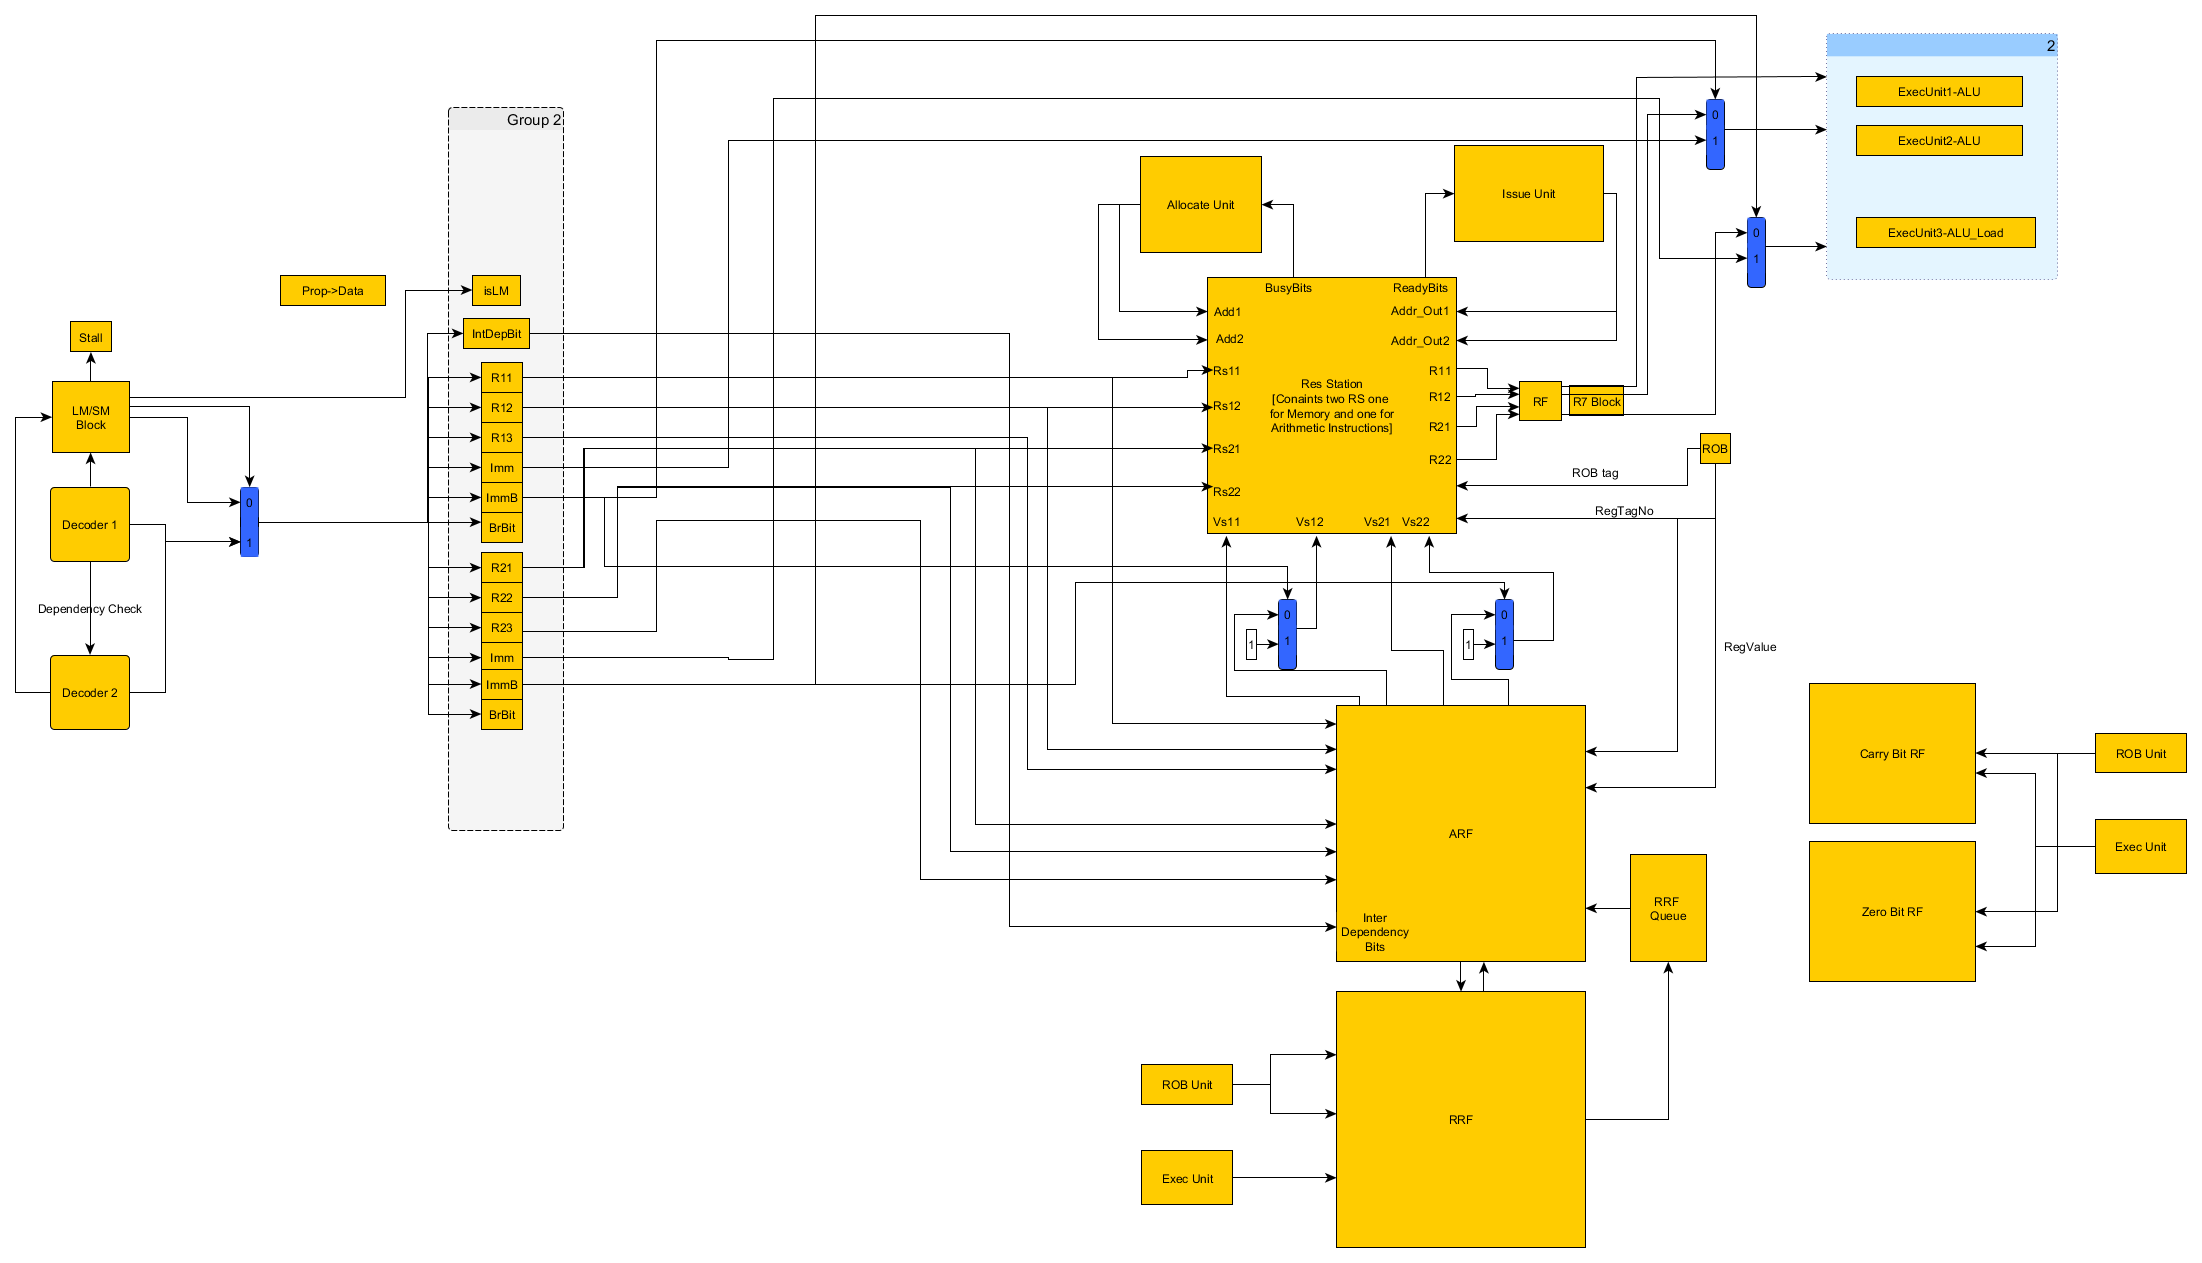
\includegraphics[scale = 0.2]{../GraphImages/dispatch_stage_arf_rrf.png}
\end{figure}

\subsection{Register Renaming}
Registers are 16-bit.
Carry and Zero Flag registers are 1-bit.
Renaming is performed for both the registers individually.
\subsubsection{Architectural Register File}
\begin{itemize}
\item They store tags of the corresponding rename regiser for every Architectural registers, along with non-speculative data.
\item It will also have a valid bit. Whenever an interrupt or flush in the ROB occurs all valid bits are set to 1.
\item If the AR is renamed, then it is invalid, else it is valid.
\item It is set valid, only when the tag pointed by it, and the tag broadcasted by the ROB matches.
\item It will take into account the interdependency bits and use the RRF queue to decide which tags to issue and which to be provided to the 
reservation station in case of a intra RAW hazard.
\end{itemize}
\subsubsection{Rename Register File}
\begin{itemize}
\item Execution will give the tag for the RR, and the corresponding register will update its value.
\item This will also be broadcasted RS.
\end{itemize}
\subsubsection{RRF Queue}
\begin{itemize}
\item Queue of available rename registers, updated based on ROB tag broadcast.
\end{itemize}
\subsection{Reservation Station}
The reservation station is maintained as a hybrid b/w the distributed and central system. One reservation station handles the ALU operations and the other handles memory based instructions. The policies for each are different and they are explained below
\subsubsection{Allocation Policy}
\begin{itemize}
\item Arithmetic (Branch) RS
\begin{itemize}
\item Keep a queue (circular), to store the available RS entries for allocation.
\item This has to check whether or not to stall.
\item The register values are from the pipeline registers, valid bits from the ARF, and ROB tag from ROB.
\item It also allocates to the ROB, and checks for stalls.
\end{itemize}
\item Memory (Branch) RS
\begin{itemize}
\item For the memory instructions becuase they are supposed to executed in order becuase we do not have load bypassing or load dependency checks, we must excute the loads and the stores strictly in order
\item Hence the allocation is performed like in a FIFO, new entries are inserted after the last tail entry
\end{itemize}
\end{itemize}
\subsubsection{Issue Policy}
\begin{itemize}
\item Arithmetic (Branch) RS
\begin{itemize}
\item Top-down search for ready bits.
\item Decides between the two ALU pipes and sends NOP(s) if (an) instruction(s) is/are not available
\end{itemize}
\item Memory (Branch) RS
\item Issue is performed only if the the top queue entry is ready. A NOP is issued otherwise.
\item This is again necessary to maintain and loads and stores in order
\end{itemize}
\subsubsection{Table Entries}
\begin{itemize}
\item Source Rename Register Tags.
\item Source Register Values and Immediate Data
\item Destination Rename Register Tags
\item ROB tag
\item Control Signals including invalidTag bits
\end{itemize}
\subsubsection{LM/SM Handling Additions}
\begin{itemize}
\item These additions are only made to the memory RS. This is not duplicated for every entry but is only one of its kind in the entire RS
\item Registers are necessary to store the tag as well as the value of the starting address of the LM/SM instruction
\item Storage of tag is necessary if the Address generating instruction (AGI) has not yet cleared the busy bit. This allows for the read to occur when the address is generated by the execution units
\item Storing the value is necessary because, once the AGI exits the ROB, the register tag stored would enter the RRF Queue and the value may be replaced which would lead to the remaining LM instructions reading the wrong instructions. And hence once the value has been written to the RRF, it is simultaneously written to this value store register (VSR) and a valid bit alongside is set to say that the value in the VSR is valid and that the tag must not be read anymore.
\end{itemize}

\section{Execution}
\begin{figure}[H]
	\centering
	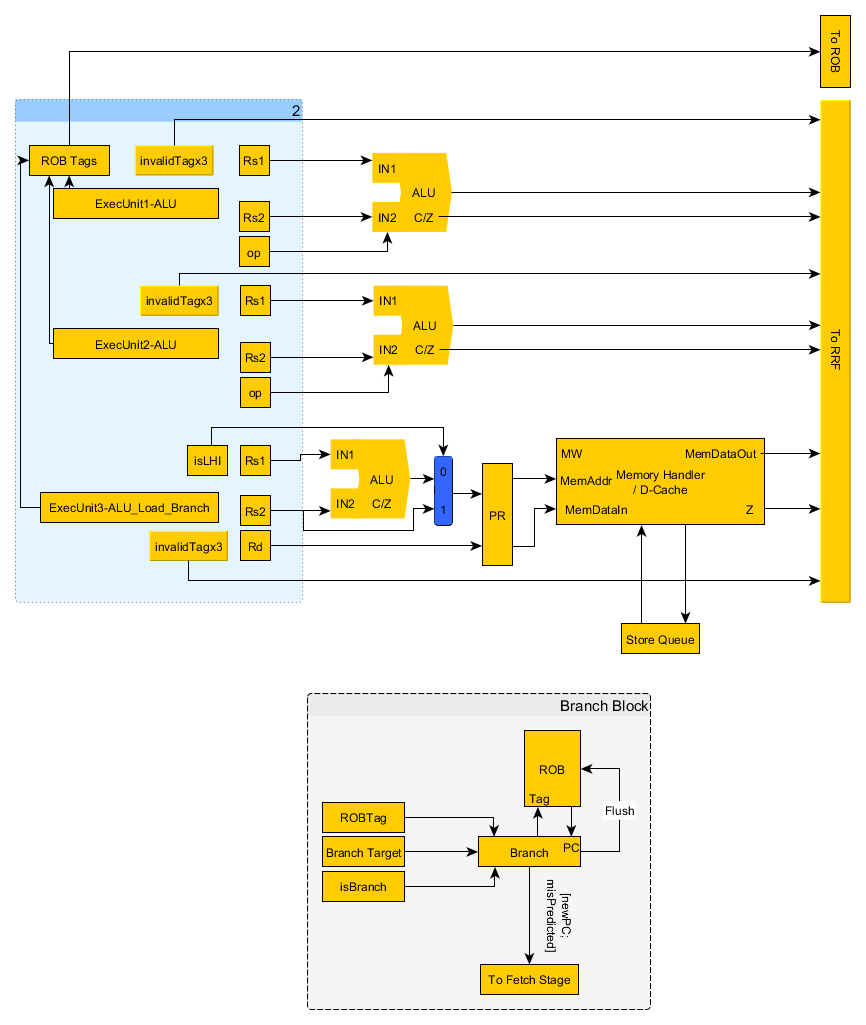
\includegraphics[scale = 0.5]{../GraphImages/execution_stage.png}
\end{figure}

\subsection{3 Pipes}
The execution unit has one memory pipe which also handles the memory based R7 write branches and two arithmetic and branch pipes
\subsection{Arithemetic/Branch Pipes}
\begin{itemize}
\item Both the pipes are copies of each other
\item They consist of an ALU which peforms the necessary operation based on the control signals and the values provided to it as an operands which are decided in the decode stage itself
\item This pipe also contains a branch handling unit which updates the speculative PC based on the data produced and if the instruction was a branch instruction. It also send the necessary flush command to the ROB
\end{itemize}
\subsection{Memory Pipe}
\begin{itemize}
\item This too consits of a similar branch unit along with the memory block. This pipeline has two stages to account for the memory read and address generation
\item Loads must also check in the Store Queue present in the write back stage, whether the data has been written or is to be written by any store to the address it must read from and perform the appropriate forwarding
\end{itemize}

\section{Write Back}
\begin{figure}[H]
	\centering
	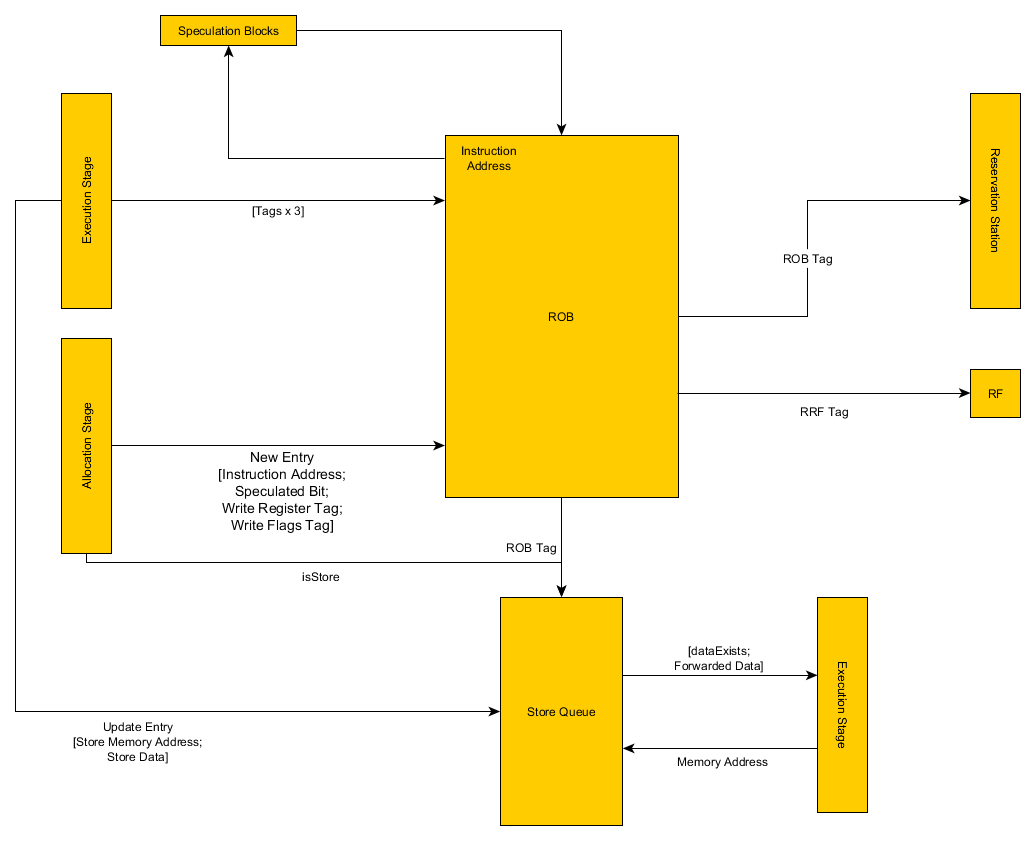
\includegraphics[scale = 0.43]{../GraphImages/writeBack_stage.png}
\end{figure}

\subsection{Reorder Buffer (ROB)}
The re-order buffer is implemented as a circular buffer, with head and tail pointers. The head pointer helps in deciding which instructions to retire and the comparison of the head and tail pointer decide when to call for a stall when the ROB get full. \\ \\
Every cycle 3 of the ROB Tags are set to finished based on the 3 bits which signify the validity of the tags (for example a tag is invalid if it was NOP instruction)
\subsubsection{Table Entries}
\begin{itemize}
\item Instruction Address
\item Destination Tag of Flags and Register
\item Invalid Tag Bits for Flags and Register
\item Speculative Bit and Valid Bit
\item Finished Bit
\end{itemize}
\subsection{Store Queue}
Store Queue is maintained to allow for lazy write. We cannot directly write to memory in the execution stage becuase writing to memory is permanent. Instead this queue acts as the temporary memory and data is marked as finished when the store instruction pops out of the ROB and then the data is forwarded to any loads that require the load till the data is written to the memory.
\end{document}
